% !TEX root = exam.tex
\newcommand{\deriv}[2]{\frac{\partial #1}{\partial #2}}

\newcommand{\backpropStudSolA}{
\begin{align*}
\sigma(x)&=\frac{1}{1+e^{-x}}\\
\frac{\partial \sigma(x)}{\partial x}&=\frac{\partial }{\partial x}\frac{1}{1+e^{-x}}\\
&=\frac{e^{-x}}{(1+e^{-x})^2}\\
&=\frac{1}{1+e^{-x}}\frac{e^{-x}}{1+e^{-x}}\\
&=\sigma(x)\frac{1+e^{-x}-1}{1+e^{-x}}\\
&=\sigma(x)(\frac{1+e^{-x}}{1+e^{-x}}-\frac{1}{1+e^{-x}})\\
&=\sigma(x)(1-\sigma(x))\\
\end{align*}
}

\newcommand{\backpropStudSolB}{
\begin{align*}
c_k &= g(h_k) \\
\delta_k &= \deriv{E}{h_k} \\
&= \deriv{}{h_k} (\frac{1}{2}\sum_{k}(c_k-t_k)^2) \\
&= \sum_{k}\big((c_k-t_k)g'(h_k)\big) \\
\end{align*}
}

\newcommand{\backpropStudSolC}{
\begin{align*}
h_k &= \sum_{j}(w_{jk}b_{j}) + f_{k} \\
\deriv{E}{w_{jk}} &= \deriv{E}{h_k} \deriv{h_k}{w_{jk}} \\
&=\delta_k \deriv{h_k}{w_{jk}} \\
&=\delta_k \deriv{}{w_{jk}}\big(\sum_{j}(w_{jk}b_{j}) + f_{k}\big) \\
&=\delta_k \sum_{j}b_{j} \\
\end{align*}
}

\newcommand{\backpropStudSolD}{
\begin{align*}
h_k &= \sum_{j}(w_{jk}b_{j}) + f_{k} \\
\deriv{E}{f_{k}} &= \deriv{E}{h_k} \deriv{h_k}{f_{k}} \\
&=\delta_k \deriv{h_k}{f_{k}} \\
&=\delta_k \deriv{}{f_{k}}\big(\sum_{j}(w_{jk}b_{j}) + f_{k}\big) \\
&=\delta_k \\
\end{align*}
}

\newcommand{\backpropStudSolE}{
\begin{align*}
h_k &= \sum_{j}(w_{jk}b_{j}) + f_{k} \\
\deriv{h_k}{b_j} &= \sum_{j}w_{jk} \\
\end{align*}
\begin{align*}
b_j &= g(z_j) \\
\psi_j &= \deriv{E}{z_j} \\
&= \deriv{E}{h_k} \deriv{h_k}{b_j}  \deriv{b_j}{z_j}  \\
&= \delta_k \sum_{j}\big(w_{jk} g'(z_j)\big) \\
\end{align*}
}

\newcommand{\backpropStudSolF}{
\begin{align*}
z_j &= \sum_{i}(u_{ij}a_{i}) + e_j \\
\deriv{E}{u_{ij}} &= \deriv{E}{z_j} \deriv{z_j}{u_{ij}} \\
&=\psi_j \deriv{z_j}{u_{ij}}\\
&=\psi_j \deriv{}{u_{ij}}\big(\sum_{i}(u_{ij}a_{i}) + e_j\big) \\
&=\psi_j \sum_{i}a_{i} \\
\end{align*}
}

\newcommand{\backpropStudSolH}{
\begin{align*}
z_j &= \sum_{i}(u_{ij}a_{i}) + e_j \\
\deriv{E}{e_j} &= \deriv{E}{z_j} \deriv{z_j}{e_j} \\
&=\psi_j \deriv{z_j}{e_j}\\
&=\psi_j \deriv{}{e_j}\big(\sum_{i}(u_{ij}a_{i}) + e_j\big) \\
&=\psi_j \\
\end{align*}
}

 %The students have to fill this file to print the solution

% Problem Explanation:
% - first argument is the number of points
% - second argument is the title and the text
\examproblem{8}{Backpropagation
}


Consider the deep net in the figure below consisting of an input layer, an output layer, and a hidden layer. The feed-forward computations performed by the deep net are as follows: every input $a_{i}$ is multiplied by a set of fully-connected weights $u_{ij}$ connecting the input layer to the hidden layer. The resulting weighted signals are then summed and combined with a bias $e_{j}$. This results in the activation signal $z_{j}=e_{j}+\sum_{i}a_{i}u_{ij}$. The hidden layer applies activation function $g$ on $z_{j}$ resulting in the signal $b_{j}$.  In a similar fashion, the hidden layer activation signals $b_{j}$ are multiplied by the weights connecting the hidden layer to the output layer $w_{jk}$, a bias $f_{k}$ is added and the resulting signal $h_{k}$ is transformed by the output activation function $g$ to form the network output $c_{k}$. The loss between the desired target $t_{k}$ and the output $c_{k}$ is given by the MSE: $E= \frac{1}{2} \sum_{k} (c_{k}-t_{k})^{2}$, where $t_{k}$ denotes the ground truth signal corresponding to $c_{k}$. Training a neural network involves determining the set of parameters $\theta=\{\emph{U},\emph{W},\emph{e},\emph{f}\}$ that minimize $E$. This problem can be solved using gradient descent, which requires determining $\frac{\partial E}{\partial \theta}$ for all $\theta$ in the model.


\begin{center}
 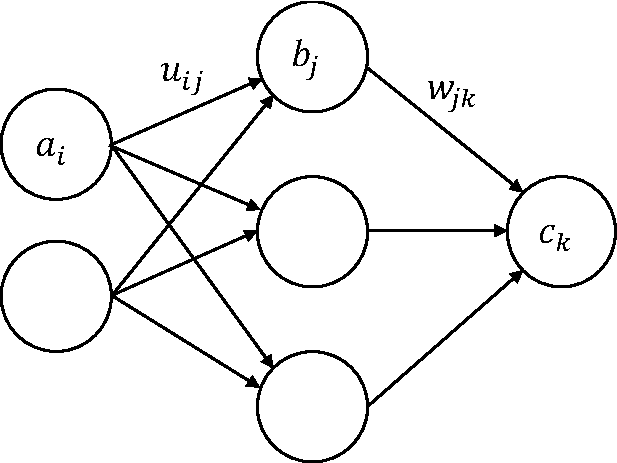
\includegraphics[width=7cm]{fig/DeepNet.pdf}
 \end{center}

%%%%%%%%%%%%%%%%%%%%%%%%%%%%%%%%%%%%%%
%%%%%  BEGINNING OF SUBPROBLEMS LIST
\begin{enumerate}

% Subproblem description
\examproblempart{ For $g(x)=\sigma(x)=\frac{1}{1+e^{-x}}$, compute the derivative $g'(x)$ of $g(x)$ as a function of $\sigma(x)$.}
\bookletskip{0}   %in inches

% Solution box 
 \framebox[14.7cm][l]{
 \begin{minipage}[b]{14.7cm}
\inbooklet{Your answer: \backpropStudSolA}
  
 \solution{\backpropSolA}

 \end{minipage}
 }

% Subproblem description
\examproblempart{ We denote by $\delta_{k}=\frac{\partial E}{\partial h_{k}}$ the error signal of neuron $k$ in the second linear layer of the network. Compute $\delta_{k}$ as a function of $c_k$, $t_k$, $g'$ and $h_k$.\\ }
\bookletskip{0}   %in inches

% Solution box 
 \framebox[14.7cm][l]{
 \begin{minipage}[b]{14.7cm}
\inbooklet{Your answer: \backpropStudSolB}
  
 \solution{\backpropSolB}

 \end{minipage}
 }

% Subproblem description
\examproblempart{ Compute $\frac{\partial E}{\partial w_{jk}}$. Use $\delta_k$ and $b_j$.\\}
\bookletskip{0.0}   %in inches

% Solution box 
 \framebox[14.7cm][l]{
 \begin{minipage}[b]{14.7cm}
 \inbooklet{Your answer: \backpropStudSolC}
  
 \solution{\backpropSolC}
  \end{minipage}
  }

% Subproblem description
\examproblempart{Compute $\frac{\partial E}{\partial f_{k}}$. Use $\delta_{k}$.\\}
\bookletskip{0.0}   %in inches

% Solution box 
 \framebox[14.7cm][l]{
 \begin{minipage}[b]{14.7cm}
 \inbooklet{Your answer: \backpropStudSolD}
  
 \solution{\backpropSolD}
 \end{minipage}
 }

% Subproblem description
\examproblempart{We denote by $\psi_{j}=\frac{\partial E}{\partial z_{j} }$ the error signal of neuron $j$ in the first linear layer of the network. Compute $\psi_{j}$ as a function of $\delta_{k}$, $w_{jk}$, $g'$ and $z_{j}$.\\ }
\bookletskip{0}   %in inches

% Solution box 
 \framebox[14.7cm][l]{
 \begin{minipage}[b]{14.7cm}
 \inbooklet{Your answer: \backpropStudSolE}
  
 \solution{\backpropSolE}
 \end{minipage}
 }
 
 
 % Subproblem description
\examproblempart{Compute $\frac{\partial E}{\partial u_{ij}}$. Use $\psi_{j}$ and $a_i$.\\ }
\bookletskip{0}   %in inches

% Solution box 
 \framebox[14.7cm][l]{
 \begin{minipage}[b]{14.7cm}
 \inbooklet{Your answer: \backpropStudSolF}
  
 \solution{\backpropSolF}
 \end{minipage}
 }
 
 
  % Subproblem description
\examproblempart{Compute $\frac{\partial E}{\partial e_{j}}$. Use $\psi_{j}$.\\ }
\bookletskip{0}   %in inches

% Solution box 
 \framebox[14.7cm][l]{
 \begin{minipage}[b]{14.7cm}
 \inbooklet{Your answer: \backpropStudSolH}
  
 \solution{\backpropSolH}
 \end{minipage}
 }
 
 
 %%%%%%%%%%%% END OF SUBPROBLEMS LIST

\end{enumerate}